\documentclass[10pt]{beamer}

%%%%% all the nerdy stuff
\usetheme{metropolis}
\usepackage{appendixnumberbeamer}

\usepackage{booktabs}
\usepackage[scale=2]{ccicons}

\usepackage{pgfplots}
\usepgfplotslibrary{dateplot}

\usepackage{outlines}

\usepackage{xcolor}

\usepackage{amsmath}

\usepackage[round]{natbib}

\usepackage{xspace}
\newcommand{\themename}{\textbf{\textsc{metropolis}}\xspace}

%%%%% title page

\title{The Impact of Trade Liberalization on Gross Exports and Domestic Value Added}
\subtitle{Mid-Course Assignment in Trade Policy Analysis}
\date{24th of November 2022}
\author{Gero Dasbach, Yangfan Tan and Alessia Tonetto}
\institute{}
\titlegraphic{\hfill\includegraphics[height=1.5cm]{logo.png}}


%%%%% the real stuff

\begin{document}

%%%% define some colors

\definecolor{mDarkViolet}{HTML}{8c62ec}
\definecolor{mLightRose}{HTML}{ec6277}
\definecolor{mChallengeRed}{HTML}{e9122c}

%%%%% title page 

\maketitle

%%%%% table of content slide
%% shows everything under \section{}

\begin{frame}{Table of contents}
  \setbeamertemplate{section in toc}[sections numbered]
  \tableofcontents[hideallsubsections] % show only most important
\end{frame}

%%%%% presentation starts from here:

\section{Introduction}

\begin{frame}[fragile]{Introduction}

\textbf{Research Question}: Was the effect of trade liberalization policies between 2002 and 2014 stronger on gross exports or on domestic value added (DVA) in gross exports?

\textbf{Motivation}:
\begin{itemize}
    \item Significant increase in RTAs: from 28 in 1990 to 355 in 2021
	\item \texttt{Time frame:} 2002-2014, captures integration into GVCs (e.g. EU enlargement 2004)
\end{itemize}

\textbf{Data}: Decomposition of WIOD trade data from the 2016 release (\cite{timmer2015illustrated}) following \cite{borin2019measuring}

\textbf{Strategy}: Obtain figures on gross exports and DVA and regress both trade measures on trade policy dummy variables and set of controls

\end{frame}

\begin{frame}[fragile]{Increase in Trade}
  \begin{figure}[h]
    \caption{GVC-related trade compared to Traditional Trade. Source: WITS}
    \centering
    \includegraphics[width=1\textwidth]{gvctrade}
\end{figure}
\end{frame}

\section{Literature}

\begin{frame}[fragile]{Literature}

 Existing Literature
      \begin{itemize}
        \item Trade creation and trade disruption: RTAs are able to increase the welfare of the region in which they are implemented (\cite{baier2007free}, \cite{mayer2019cost}) 
	\item Determinants of effects of trade: geographical location, economic size, political ties (\cite{felbermayr2018schengen}, \cite{felbermayr2022complex}, \cite{baier2019putting})
	\item \textbf{Existing gap in the literature}: The existing literature does not address the question if reshoring which follows economic disintegration is linked to increased domestic value added!
	\item Given the complexity of \textbf{GVC}, it is now vital to account for the different components of the value added generated by trade (\cite{antras2021global}, \cite{aslam2017calculating}). \cite{koopman2014tracing} provides an insightful decomposition of gross exports that takes into account both the created value added and the vertical specialization
      \end{itemize}

\end{frame}

%%%%%%%%%%%%%%%%%%%%%%%%%%%%%%%%%%%%%%%%%   Gero  %%%%%%%%%%%%%%%%%%%%%%%%%%%%%%%%%%%%%

\section{Data and Specifications}

\begin{frame}{Data i}
    \begin{alertblock}{Gross exports and DVA}
      \begin{outline}
    \1 Source: WIOD 2016 release, decomposition scheme as in \cite{borin2019measuring}
          \2 Gross exports (GTRADE) in million USD
          \2 Domestic value added (DVA) in million USD
      \end{outline}
    \end{alertblock}
      
    \begin{block}{Trade liberalization policy}
       \begin{outline}
          \1 Source: Larch's RTA database (\cite{egger2008interdependent})
           \2 RTA dummies capture seven different FT policies: 
           \textit{CU, FTA, PSA, EIA, CUEIA, FTAEIA, PSAEIA}
           \3 e.g. \textit{EIA} captures the EU, \textit{CU} captures EU-TUR CU (1995), \textit{FTAEIA} captures NAFTA (1993), EU-MEX (2000), EU-KOR (2011)
      \end{outline}
    \end{block}
      
    \begin{exampleblock}{Controls}
    \begin{outline}
          \1 Source: CEPII GRAVITY database (\cite{conte2022cepii})
          \2 Standard gravity dummies capture several controls for endogeneity: \textit{Distance, Border, Language, Colony}
      \end{outline}
    \end{exampleblock}
\end{frame}

\begin{frame}{Data ii} 
\textbf{Trade liberalization policy dummies}
\begin{columns}
\column{0.75\textwidth}
      \begin{figure}
    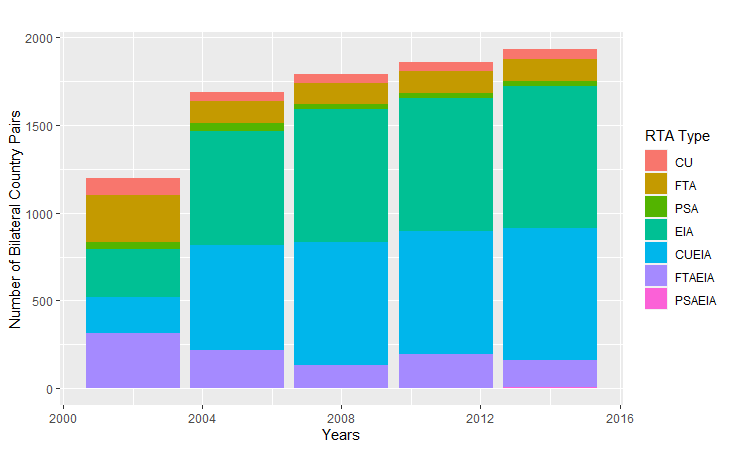
\includegraphics[scale=0.4]{graph_1a.png} % scale = 0.9 means 90%, can adjust
    \small{\caption{The RTA policy dummies (2002-2014). Information on RTAs from 
    \href{http://rtais.wto.org/UI/PublicMaintainRTAHome.aspx}{WTO's RTA database}.}}
  \end{figure}
  
\column{0.25\textwidth}
    \begin{itemize}
          \item \color{mLightBrown}{e.g. EU-TUR CU (1995) $\in$ \textit{CU}}
          \item \color{mLightGreen}{e.g. EU $\in$ \textit{EIA}}
          \item \color{mDarkViolet}{e.g. NAFTA (1993), EU-MEX (2000), EU-KOR (2011) $\in$ \textit{FTAEIA}}
    \end{itemize}
\end{columns}
\end{frame}

\begin{frame}{Data iii} 
\begin{columns}
    \column{0.80\textwidth}
      \begin{figure}
    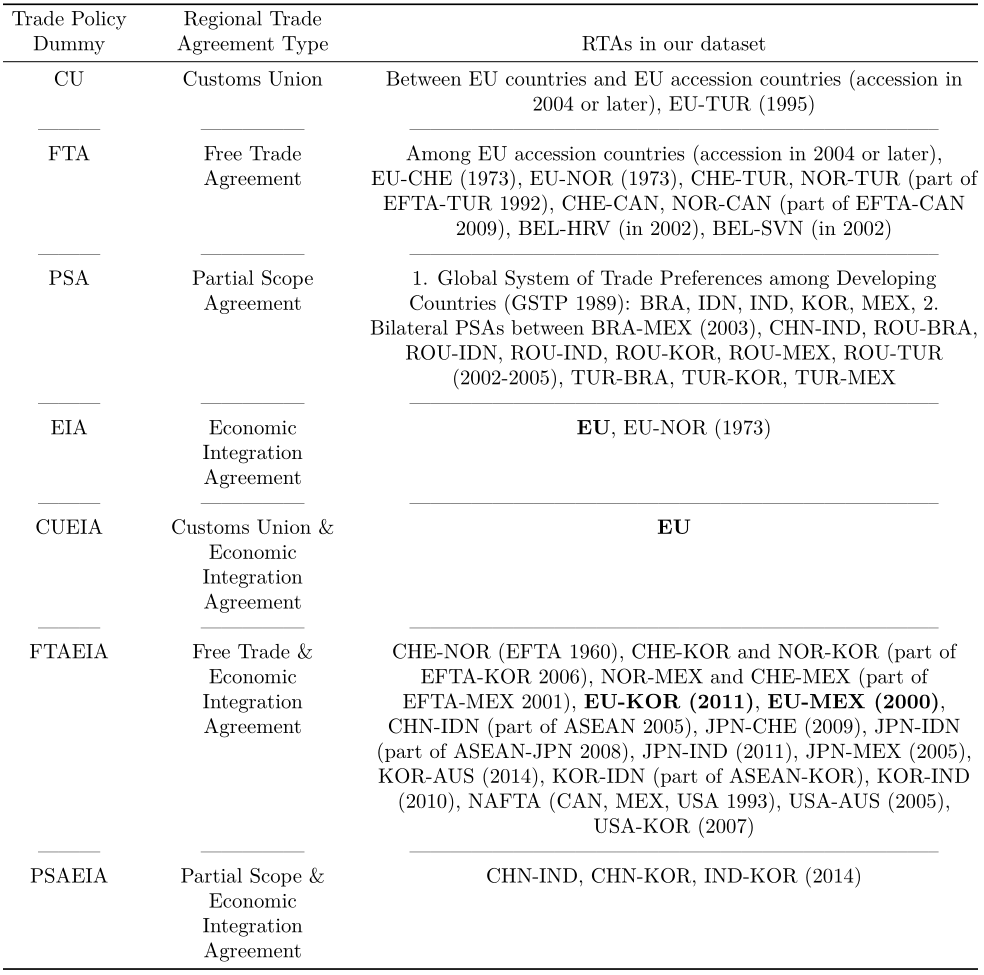
\includegraphics[scale=0.4]{data_rta.png} % scale = 0.9 means 90%, can adjust
    \caption{}
      \end{figure}
    \column{0.20\textwidth}
    \textbf{Figure 3:}The RTA policy dummies (2002-2014). \\ Information on RTAs from 
    \href{http://rtais.wto.org/UI/PublicMaintainRTAHome.aspx}{WTO's RTA database}.
\end{columns}
\end{frame}

{
    \metroset{titleformat frame=smallcaps} % default setting
\begin{frame}{Data Wrangling}
\begin{columns}
\column{0.40\textwidth}
      \begin{figure}
    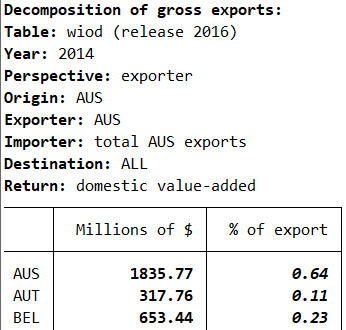
\includegraphics[scale=0.6]{icio_dva.png} % scale = 0.9 means 90%, can adjust
    \small{\caption{The icio command helps to extract DVA in gross exports.
    \href{http://www.tradeconomics.com/icio/}{More on the command here.}}}
  \end{figure}

\column{0.60\textwidth}
\begin{enumerate}
    \item Extract WIOD 2016 data on gross exports (GTRADE) and DVA: STATA icio command by \cite{belotti2020icio}
    \item Merge both datasets on GTRADE and DVA with the RTA and GRAVITY datasets
    \item Perform gravity regressions on final dataset
\end{enumerate}
\end{columns}
\end{frame}
}


\begin{frame}{Estimation Challenges and Specifications}
\begin{alertblock}{\color{mChallengeRed}{Estimation Challenges}}
    \begin{outline}
    \1 Our \textbf{four specifications} tackle different econometric challenges
    \2 \textbf{(i)}: OLS estimator with absorbed importer-time and exporter-time FE
    \2 \textbf{(ii-iv)}: PPML estimator with absorbed importer-time and exporter-time FE
    \3 \textbf{(iii)}: intra-national trade to account for home bias
    \3 \textbf{(iv)}: exporter-time and importer-time and exporter-importer pair FE to account for endogeneity
    \end{outline}
\end{alertblock}

\begin{alertblock}{\color{mLightGreen}{Solutions}}
    \begin{figure}
    \includegraphics[scale=0.25]{model_estimation.PNG} % scale = 0.9 means 90%, can adjust
    \tiny{\caption{How we tackle estimation challenges defined in \cite{yotov2016advanced}}}
   \end{figure}
\end{alertblock}

\end{frame}


\begin{frame}{Specifications (i)-(iv)}

\textbf{Specification (ii): PPML estimator}

\begin{enumerate}
    \item 
\begin{math}\label{eq:1}
\color{mLightBrown}{GTRADE_t^{ij}} \color{mDarkTeal}{= \alpha +} \color{mLightGreen}{\beta GRAVITY^{i}} \color{mDarkTeal}{+ \gamma_1 CU + \gamma_2 FTA + \gamma_3 PSA +  \gamma_4 EIA +\\ \gamma_5 CUEIA +  \gamma_6 FTAEIA+  \gamma_7 PSAEIA} + \color{mLightRose}{\mu_t^{i} + \eta_t^j + \epsilon_t^{ij}}
\end{math}

\item 
\begin{math}\label{eq:2}
\color{mLightBrown}{DVA_t^{ij}}  \color{mDarkTeal}{= \alpha +} \color{mLightGreen}{\beta GRAVITY^{i}} \color{mDarkTeal}{+ \gamma_1 CU + \gamma_2 FTA + \gamma_3 PSA +  \gamma_4 EIA +\\ \gamma_5 CUEIA +  \gamma_6 FTAEIA+  \gamma_7 PSAEIA} + \color{mLightRose}{\mu_t^{i} + \eta_t^j + \epsilon_t^{ij}}
\end{math}
\end{enumerate}

\textbf{Specification (iii): Home bias with the PPML estimator}

\begin{enumerate}
    \item 
\begin{math}\label{eq:3}
\color{mLightBrown}{GTRADE_t^{ij}} \color{mDarkTeal}{= \alpha +} \color{mLightGreen}{\beta GRAVITY^{i}} \color{mDarkTeal}{+ \gamma_1 CU + \gamma_2 FTA + \gamma_3 PSA +  \gamma_4 EIA +\\ \gamma_5 CUEIA +  \gamma_6 FTAEIA+  \gamma_7 PSAEIA} + \color{mLightRose}{\delta INTRA  + \sigma_t^i + \theta_t^j + \psi^{ij} + \epsilon_t^{ij}}
\end{math}

\item 
\begin{math}\label{eq:4}
\color{mLightBrown}{DVA_t^{ij}} \color{mDarkTeal}{= \alpha +} \color{mLightGreen}{\beta GRAVITY^{i}} \color{mDarkTeal}{+ \gamma_1 CU + \gamma_2 FTA + \gamma_3 PSA +  \gamma_4 EIA +\\ \gamma_5 CUEIA +  \gamma_6 FTAEIA+  \gamma_7 PSAEIA} + \color{mLightRose}{\delta INTRA  + \sigma_t^i + \theta_t^j + \psi^{ij} + \epsilon_t^{ij}}
\end{math}
\end{enumerate}
\end{frame}


%%%%%%%%%%%%%%%%%%%%%%%%%%%%%%%%%%%%%                    %%%%%%%%%%%%%%%%%%%%%%%%%%%%%%%%%%%%%%

\section{Results and Discussion}

\begin{frame}{Results i}
    \begin{figure}
    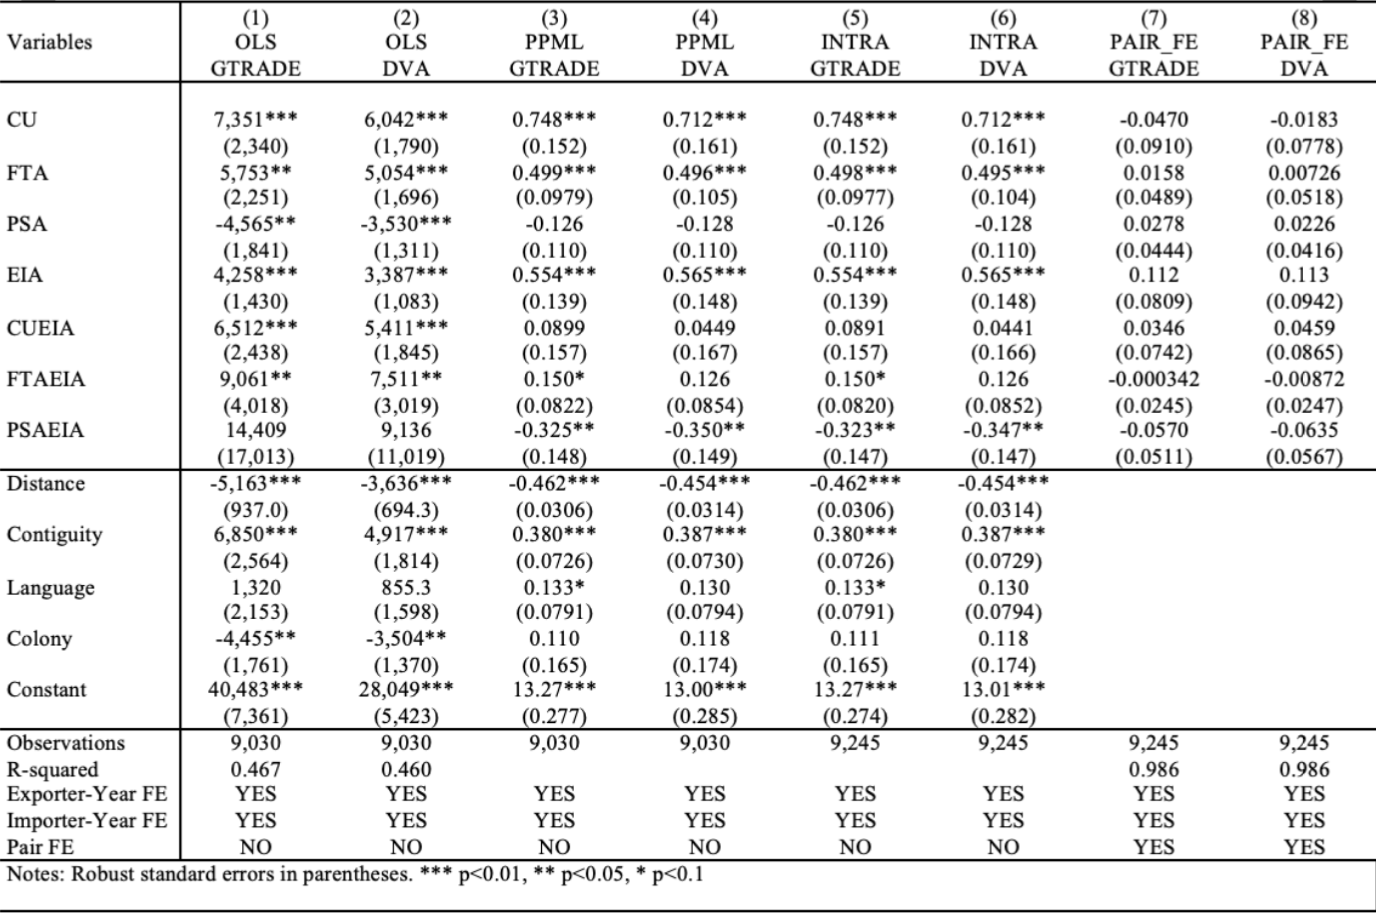
\includegraphics[scale=0.4]{results.PNG} 
    \tiny{\caption{The results of specifications (i)-(iv) for both trade measures.}}
    \end{figure}
\end{frame}
    
\begin{frame}{Results ii}
\textbf{Columns (1) and (2)}:
\begin{itemize}
    \item Estimated results for the baseline gravity equation (i) by OLS
    \item CU, FTA, EIA, CUEIA, and FTAEIA: significant  positive  effects on bilateral trade flows, both measured by GTRADE and DVA
    \item PSA has significant negative effects and no significant effects of PSAEIA
    \item GTRADE vs DVA: the former has a larger absolute magnitude in all coefficient estimates, suggesting the trade agreement variables have larger effects on GTRADE than DVA
\end{itemize}

\textbf{Columns (3) and (4)}:
\begin{itemize}
    \item Estimated results for the baseline gravity equation (i) by PPML
    \item Significantly positive effects of CU, FTA, and EIA. CUEIA and FTAEIA lose significance. PSAEIA has significantly negative effects
    \item Absolute magnitude of effects is larger on GTRADE than DVA
\end{itemize}
\end{frame}

\begin{frame}{Results ii}
\textbf{Columns (5) and (6)}:
\begin{itemize}
    \item Estimated results for the gravity equation (iii) controlling for intra-national trade by PPML. 
    \item The results are similar to those estimated for equation (1), besides some slight decrease in absolute magnitude. 
\end{itemize}

\textbf{Columns (7) and (8)}:
\begin{itemize}
    \item Estimated results for the gravity equation (iv) controlling for endogeneity by PPML
    \item NO significant results at all
\end{itemize}
\end{frame}

\begin{frame}{Discussion}
\textbf{Trade liberalization and aggregate trade flows}:
\begin{outline}
    \1 EU effects in comparison:
    \2 1950-2012: \cite{mayer2019cost}'s PPML yield a 300\% increase for EU trade (+6 times)
    \2 1995-2011: \cite{felbermayr2018schengen} find a 122\% increase for EU trade (+2.5 times)
    \3 Plausible explanation: rise in GVC integration in the 1990s and slowdown in GVC integration after 2014
\end{outline}

\textbf{Trade liberalization and domestic value added (DVA)}:
\begin{outline}
    \1 Coefficients on GTRADE absolutely larger than on DVA
    \1 \texttt{BUT}: In our sample, DVA/GTRADE=74\% 
    \2 DVA increasing relatively more than GTRADE: GTRADE partly driven by GVC integration
    \1 Regional GVC integration: both CU and EIA dummies $>$ FTA dummy
    \2 FTA dummy: loose FTAs, e.g. EU-NOR or EFTA-TUR vs. CU dummy: free tariffs on EU single market (2004 enlargement)
\end{outline}

%%%%%%%%%%%%%%%%%%%%%%%%%%%%%%%%%%%%%%%%%%              %%%%%%%%%%%%%%%%%%%%%%%%%%%%%%%%%%%%%

\end{frame}
\section{Conclusions}

\begin{frame}{Conclusions i}
\begin{itemize}
    \item We study the trade effects of different trade agreement regimes by adopting a set of seven trade agreement regime dummies: CU, FTA, PSA, EIA, CUEIA, FTAEIA, and PSAEIA
    \item Instead of only targeting GTRADE, we add another measure for trade flows: trade in DVA 
    \item Against the background of the international diffusion of production networks and countries’ increasing participation in GVCs over the past decades, this is a fairly interesting endeavour 
    \item Based on the icio STATA command, we extract gross bilateral trade flows and the DVA component of gross trade for 43 countries from 2002 to 2014, with an interval of three years 
\end{itemize}
\end{frame}

\begin{frame}{Conclusions ii}
\begin{itemize}
    \item By and large, we find significant and positive trade effects of CU, FTA, and EIA and that, with one exception, the absolute magnitude of effects is larger for GTRADE compared to DVA
    \item Important finding: despite smaller absolute effects of trade liberalization on DVA than on GTRADE, the relative gains to DVA are larger 
    \item Overall, the inconsistency and instability of estimates is expected given our limited data coverage, as we only include five periods and 43 countries
    \item Important limitation: aggregation over industries masks sectoral heterogeneity 
    \item Debate on welfare effects of trade liberalization get another measure: DVA
    \item Potential further questions in the light of DVA as an additional GVC measure: does DVA result in welfare gains? Who gains the most? 
\end{itemize}
\end{frame}

%%%%%%%%%%%%%%%%%%%%%%%%%%%%%%%%%%%%%%                 %%%%%%%%%%%%%%%%%%%%%%%%%%%%%%%%%%%%%

\begin{frame}[standout]
  Questions?
\end{frame}

\begin{frame}[allowframebreaks]{References} % will add "i" to first slide, etc.
  \bibliography{references.bib}
  \bibliographystyle{apalike}
\end{frame}

\appendix

\begin{frame}[allowframebreaks]{Appendix}
\begin{figure}
    \centering
    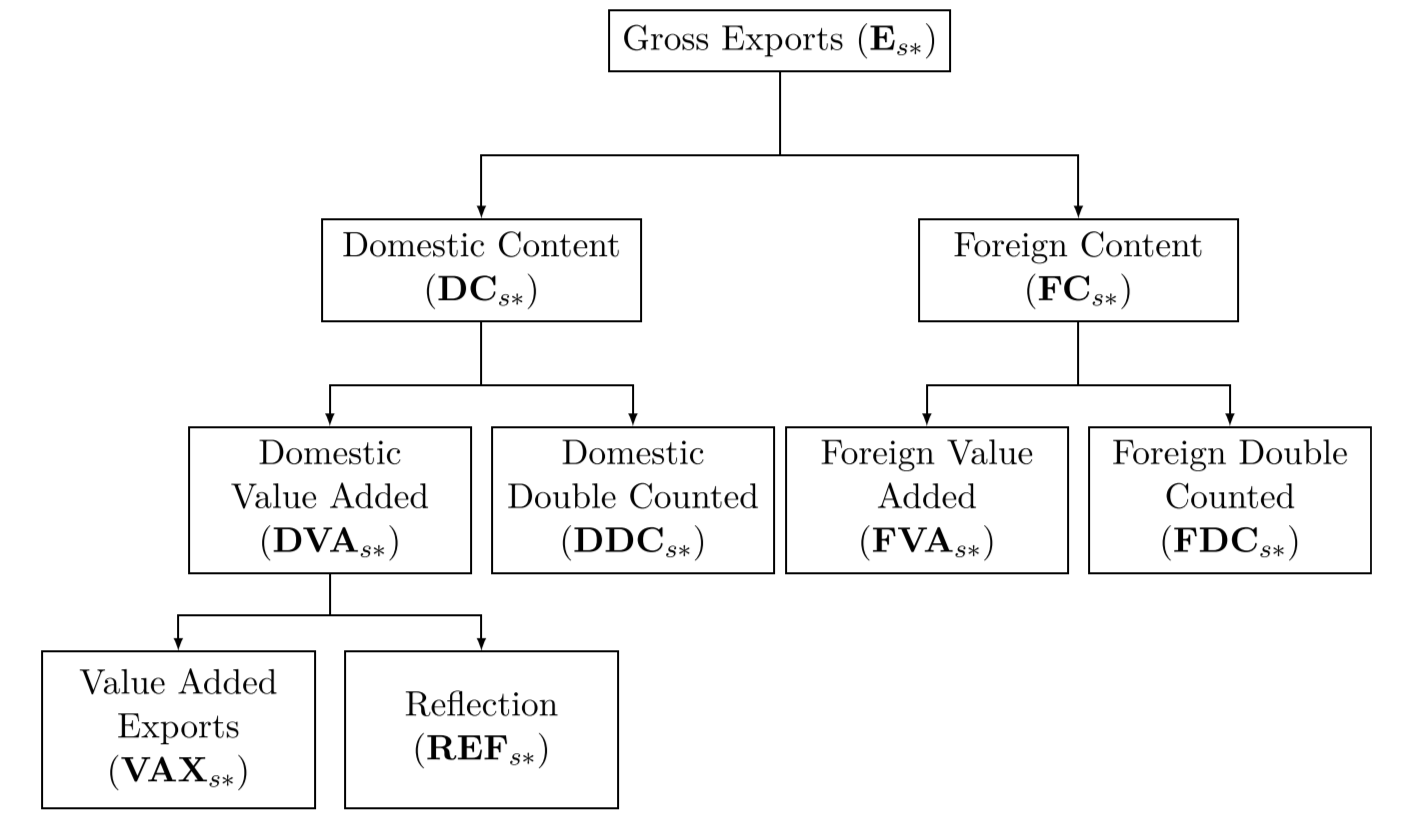
\includegraphics[scale = 0.28]{decomposition.PNG}
    \tiny{\caption{The break-down of gross exports into sub-components which \cite{borin2019measuring} adapt in their algorithm. Framework drawn from \cite{koopman2014tracing}.}}
    \label{fig:7}
\end{figure}

Please find \textbf{replication code and data} \texttt{\href{https://github.com/gerodasbach/Trade-Policy-Analysis}{here}} for download
\end{frame}


\end{document}